\documentclass[12pt]{article}

\usepackage[utf8]{inputenc}
\usepackage[letterpaper, margin=0.5in, includefoot]{geometry}
\usepackage{multicol}
\usepackage{datetime}
\usepackage{fancyhdr}
\usepackage{graphicx}
\usepackage{hyperref}
\usepackage{verbatim}
\usepackage{wrapfig}
\usepackage{CJKutf8}
\usepackage[font=small, labelfont=bf]{caption}
\usepackage{setspace}
\usepackage{tikz}
\usepackage{enumitem}
\usepackage{nameref}
\usepackage{newunicodechar}

\pagenumbering{gobble}

\newdateformat{mydate}{\dayofweekname{\the\day}{\the\month}{\the\year}, \monthname[\the\month] \the\day, \the\year}

\pagestyle{fancy}
\fancyhf{}
\cfoot{\begin{CJK}{UTF8}{min}オートセール\end{CJK} (Autocell) \hfill Bryant Benzant -- bryantbenzant@gmail.com \hfill \mydate\today}
\renewcommand{\headrulewidth}{0pt}

\newenvironment{indenteddescription}%
{\begin{list}{}{\setlength{\labelwidth}{0pt}
	\setlength{\itemindent}{-\leftmargin}
	\setlength{\listparindent}{\parindent}
	\renewcommand{\makelabel}{\descriptionlabel}}}%
{\end{list}}

\newunicodechar{¥}{\textyen}
\DeclareTextCommandDefault{\textyen}{%
	\vphantom{Y}%
	{\ooalign{Y\cr\hidewidth\yenbars\hidewidth\cr}}$\,\,$%
}
\newcommand{\yenbars}{%
	\vbox{
		\hrule height.1ex width.4em
		\kern.15ex
		\hrule height.1ex width.4em
		\kern.3ex
	}%
}

\title{Ten-Pager GDD}

\begin{document}
\begin{CJK}{UTF8}{min}
	%\doublespacing
	\begin{titlepage}
		\begin{center}
			\doublespacing
			%\includegraphics[width=7.5in]{} \\
			\textbf{\Huge Autocell \\ オートセール} \\
			\textbf{\footnotesize (ootoseeru)} \\
			Design by Bryant Benzant (Spadyal) \\
			\mydate\today \\
			For PC \& Mac \\
			\textbf{Ages:} 8 -- Up \\
			\textbf{Release Date:} July 7, 2019
		\end{center}
	\end{titlepage}
	\section*{Game Story Summary}
	Beck, the robotic humanoid, arrives to the city of the future where cars are being made. However, Beck does not have enough money to buy a car. Since this city is where they have the best auto parts than anywhere, Beck has to get some money to buy some parts all over the borough and build a car at any service stop.

	\section*{Game Flow Outline}
	\textbf{Autocell} is an open world physics-based platformer that finds Beck exploring the city and playing through levels with special physics provided as a challenge to players. The player will have a certain amount of money---the currency is bolts (as dollars) and screws (as cents)---and will have to buy auto parts to fix the car. The player will get to customize their own car with parts that they buy from real world brands: \textbf{Autozone}, \textbf{Advance Auto Parts}. Each of these parts will have a unique advantage for the player that can apply to the real world. \newline
	\begin{center}
		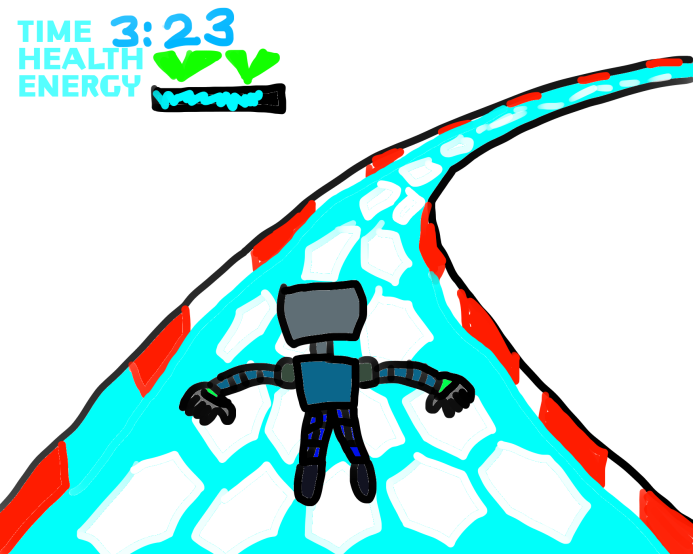
\includegraphics[width=6in]{Gameplay}
	\end{center}
	\subsection*{MARKETING PLAN}
	The main idea of \textbf{Autocell} is to get people to buy auto parts by trying out how would they work in a car. An apparatus can change depending on the parts that the player uses. This is a good marketing plan to get consumers to get into buying auto parts to make their vehicle drive better in terms of performance.
	\newpage
	\section*{CHARACTERS}
	All characters in this game are robots that have their free will---they are not programmed to do what humans made.
	\subsection*{Beck}
	A human robot with a dream to get a car that is very unique from all the other cars. He was programmed to be an assistant mechanic. Then he moved to this city not only to achieve his dream, but to be part of this city where his kind are meant to be.
	\begin{comment}
	
	\subsection*{Ryan}
	
	\subsection*{Axl}
	
	\subsection*{Kieran}
	
	\subsection*{Shye}

	\end{comment}
	\begin{center}
		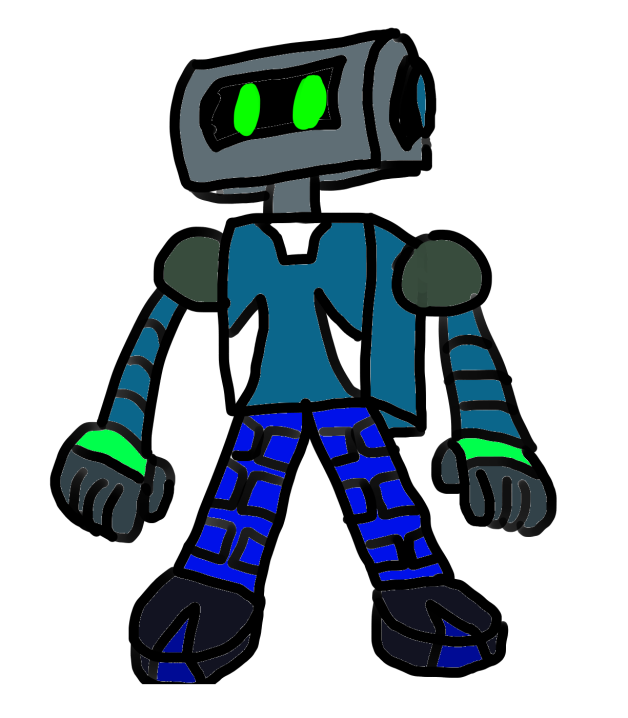
\includegraphics[width=4in]{Beck}
	\end{center}
	\section*{CONTROLS}
	\textbf{Title} uses the following keyboard (and gamepad) controls to play:
	\begin{itemize}[noitemsep]
		\item Press the arrow keys to walk
		\item Press the Space Bar Button to jump
		\item Press the Z Button to perform an attack
		\item Press the X Button to interact with people or to enter a shop
		\item Press the Backspace Button to pause
	\end{itemize}
	*\textit{Note: The player can customize the controls (both keyboard and gamepad)}
	\newpage
	\section*{GAMEPLAY}
	\textbf{Autocell} is a physics-based platformer, where the player goes to any location in the metropolis. Some physics concepts include momentum, gravity changes (staying in the ceiling or on the floor), centripetal force, and more.
	%includegraphics[width=in]{}
	\subsection*{GAME WORLD}
	Levels take place in certain locations around the city. Each of those locations contain 3 levels and a boss round. Completing those locations will grant the player a special car part and a large amount of money. \newline \newline
	\textbf{Route 6} is the first Location of \textbf{Autocell}. This is a route that varies its speed depending on the level. It includes three levels including the Highway, the Boulevard, and the Streets. \newline \newline
	\textbf{Coast Park} is the second Location of \textbf{Autocell}. This is a park located at the edge of the river. It includes three levels including the Metro Hill, Riverside Track, and Boardwalk. \newline \newline
	\textbf{Lost Tunnel} is the third Location of \textbf{Autocell}. This is a road tunnel that is a shortcut from the north area of the city to the south area. It includes three levels including Road Run, Pipe Run, and \hrulefill. \newline \newline
	\textbf{Premier Center} is the fourth Location of \textbf{Autocell}. This is a large open-air shopping center with almost all the stores and restaurants in the country. It includes three levels including the Outdoor Mall, Parking Lot, and Inner Mall. \newline \newline
	\textbf{Prime Town} is the fifth Location of \textbf{Autocell}. This is the heart of the city where the crowds are up to the limit. It includes three levels including the University, the Business Building, and the \hrulefill. \newline \newline
	\textbf{Train Flow} is the sixth Location of \textbf{Autocell}. This is the underground part of the city where the transportation is . It includes three levels including the Subway, Station Hopping Area, and the Railroad. \newline \newline
	\textbf{Carnival Tower} is the seventh Location of \textbf{Autocell}. This is a tower, each floor representing a world of attractions that is all about fun. It includes three levels including Amusement Floor, Zoo Floor, and the Night Club Floor. \newline \newline
	\textbf{Eco Airline} is the eighth Location of \textbf{Autocell}. This is the airport for flying into other robotic cities. It includes three levels including Rail Link, Gate, and Airplane. \newline \newline
	\textbf{Skyline Heights} is the ninth World of \textbf{Autocell}. This is the hotel that fellow robotic visitors can stay. It includes three levels including the Business Floor, the Boiler Room, and the Balcony Floor. \newline \newline
	\textbf{Elite Bridge} is the tenth, final, and unlockable Location of \textbf{Autocell}. This is the main landmark of the city where the robots begin their new chapter of their journey---which is also the reason why this Location is unlockable. It includes three levels including below the Road, Above the Road, and the Terminal. \newline \newline
	%\end{multicols}
	\newpage
	\begin{center}
		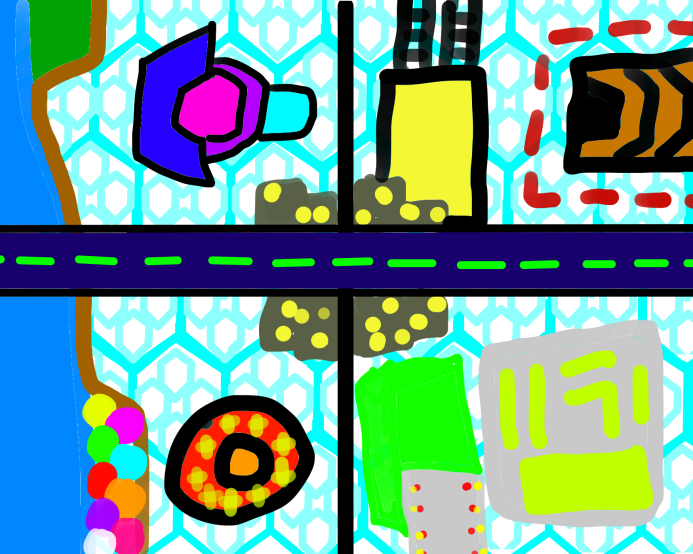
\includegraphics[width=7.5in]{Map}
	\end{center}
	\newpage
	\section*{GAME EXPERIENCE}
	After the Spadyal logo, the player is taken to the start screen. The player will have three options: New Game, Continue, and Options. New Game lets the player begin to play the game for the first time. Continue takes the player to a menu where they saved their previous progress on the game. Options lets players change the settings on the game. \newline \newline
	\noindent The beginning of the game will have the gameplay begin with Beck as the player of the game and the player can wander around or just get into the story of the game (kind of like when the player begins Zork I).
	\begin{center}
		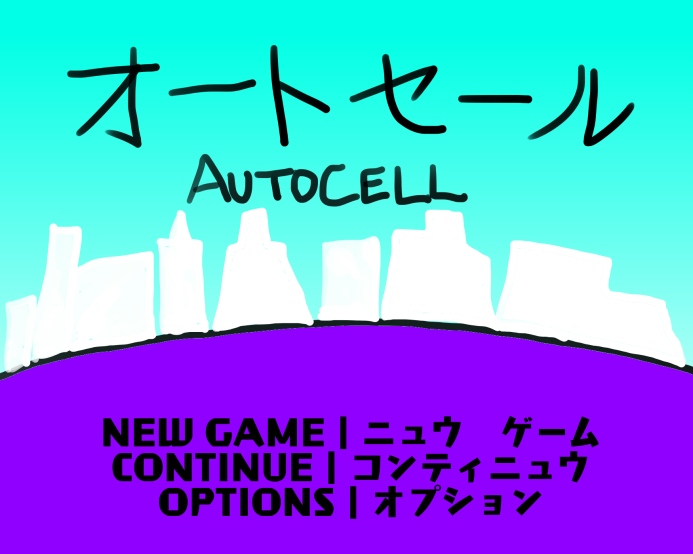
\includegraphics[width=5in]{GameExperience}
	\end{center}
	%\noindent The world and characters of \textbf{Title} \_ \newline \newline
	The music in \textbf{Autocell} should be electronic music---specifically ambient or trance. It should be something different and interesting for the player to experience the rhythmic gameplay while listening to the music in the background.
	\newpage
	\section*{GAME MECHANICS}
	There are some of the hazards, equipment, gear, tools, clothing, and food available to the player.
	\subsection*{MECHANICS / HAZARDS}
	
	\begin{multicols}{2}
		\begin{center}
			Ramming Vehicles (i.e., Cars, Trucks, Trains) \\
			Broken/Dead Neon Lights \\
			Steam Pipes \\
			Boosters \\
			Rails \\
			Fire \\
		\end{center}
	\end{multicols}
	\subsection*{EQUIPMENT / GEAR / TOOLS}
	Below are essential for the player to pass levels:
	\begin{itemize}[noitemsep]
		\item Battery
		\item Brakes \& Traction Control Systems
		\item Bumper Accessories
		\item Engine
		\item Headlamps \slash Headlights
		\item Tires
		\item Oil
		\item Wheels
		\item Exhaust
		\item Windshields
		\item Cover
		\item Electricity
		\item Plasma
		\item Seats
		\item Air Intake
		\item Lighting
		\item Speedometer
	\end{itemize}
	\begin{comment}
	\newpage
	\section*{ENEMIES}
	
	\section*{BOSSES}
	
	\begin{description}[align=right,labelwidth=3cm,noitemsep]
		\item [] \label{MechaSally}
		\item [] \label{MechaSally}
		\item [] \label{MechaSally}
		\item [] \label{MechaSally}
		\item [] \label{MechaSally}
		\item [] \label{MechaSally}
		\item [] \label{MechaSally}
		\item [] \label{MechaSally}
		\item [] \label{MechaSally}
	\end{description}
	\end{comment}
	\vfill
	\begin{center}
		\textbf{\Huge Compiled with \LaTeX}
	\end{center}
\end{CJK}
\end{document}